%!TEX root=..\master.tex
\section{Bell Lapadula}

Bell and LaPadula have devised a mathematical model intended for use in  military and governmental computer systems.
The model formalizes users accessing data and how to handle this in a secure way so confidential information cannot be leaked to a lower classification level.
The following description is based on \citet{lapadula1996secure}.

\subsection{Security}
Before we go into details about how the Bell-LaPadula (BLP) security model is applied to computer systems, we will first discuss some important concepts.

In any system we will have \textit{objects} and \textit{\subjects{}}, where objects are entities that can somehow be manipulated by the system's users (\subjects{}).
\Subjects{} can be users themselves, but can also be seen as representatives of a user or even groups of users.

\paragraph{Classification and Clearance}
Attached to any object or \subject{} will be a classification or clearance respectively.
This means that for any object $o$ with classification $x$, any \subject{} $s$ will need clearance $x$ or higher in order to access $o$.
In a hierarchical security system, where classification $y$ is a child of $x$, then an object given clearance $x$ will also have access to any objects with classification $y$.

\paragraph{Category and Need-to-know}
In addition to classification, objects can belong to zero, one or more category, which can be seen as security groupings of certain objects (e.g. ``Cold War'').
Similarly, \subjects{} can have zero, one or more need-to-know, which are the security groupings for \subjects{}.

\paragraph{Visualization}
This kind of security system can be seen as a \textit{lattice}, see \cref{blp:lattice}.
Each node represents an object, with a classification and possibly a category.
In the figure a \subject{} with the clearance \emph{Top secret} is able to read all nodes with the classification \emph{Top Secret} as well as all lower classifications (\emph{Secret} and \emph{Unclassified}).
On the contrary a \subject{} with the clearance \emph{Unclassified} can only read the one node with the \emph{Unclassified} label.

\begin{figure}
\centering
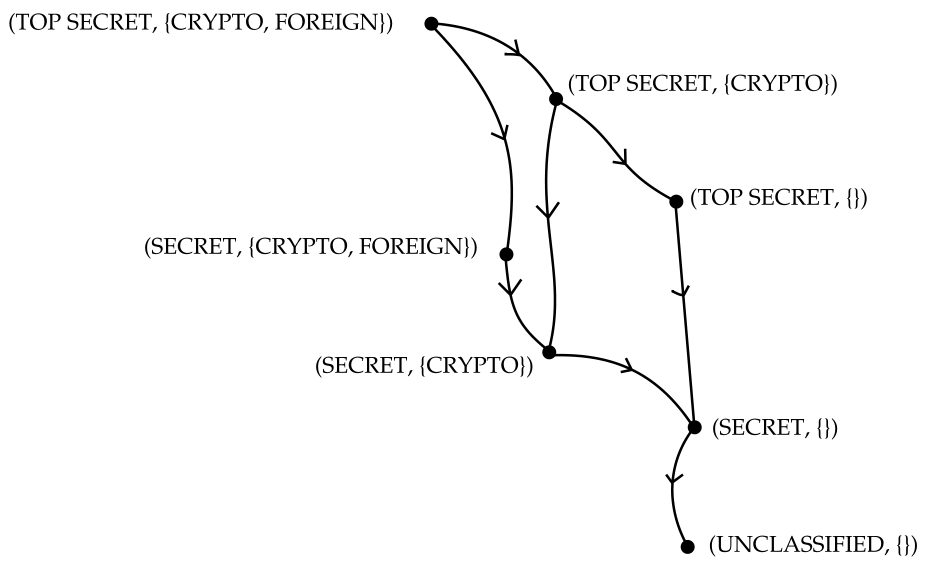
\includegraphics[width=\textwidth]{figures/blp_lattice}
\caption{A BLP lattice \cite{security_engineering_ross_anderson}}
\label{blp:lattice}
\end{figure}

\subsection{Access attributes}
The model considers four attributes for access in a complex computer system: \emph{read-only}, \emph{append}, \emph{execute} and \emph{read/write}.
In addition \emph{control access} is used to give attributes to other users.

\paragraph{Read-only}
This attribute makes it possible to read the object but not alter it.
The classical example is a file that contains information that should not be changed.
Alternatively it could be a list containing the \principals{} in the system with their clearance levels.
A \principal{} of low clearance should be able to read this list but not change it.

\paragraph{Append}
Append describes a pure write operation.
This means that it is possible to append information to the end of a file without being able to extract information about the rest of the file.

This can also be used with a printer which appends information about what is being printed.
By doing this it is sufficient that the classification of a piece of information is matching the classification of the printer in order to prevent unauthorized personnel from reading the information.

\paragraph{Execute}
The execution attribute makes it possible to execute an executable file.
If the \principal{} does not have permission to read from or write to the file he will only be able to execute it.
Similarly the executable file can produce output that is of a higher classification level than the clearance level of the \principal{} executing it.

\paragraph{Read/write}
This attribute signifies that read and write access are both allowed.
This attribute is what is traditionally used when editing text files.

\paragraph{Control access}
The control access attribute models the notion of a \principal{} having control over a file.
Having this attribute a \principal{} can give the four attributes above to other \principals{} in the system.

\subsection{Requests and decisions}
In a computer system the \principals{} are not directly accessing objects in the system, it is processes in the system that act on behalf of the \principal{}.
In the following a user requesting access to a file will be written as a \principal{} requesting access and the response to this request a decision
\bruno{Gennemgående eksempel \#57}

\subsection{Preventing security compromise}\label{bellap:properties}
In order to ensure that data cannot be compromized the previous definitions of access attributes and requests can be utilized to formalize properties that ensure that compromise cannot occur.

\paragraph{Security condition}
The security condition states that a \principal{} with a given clearance level is prevented from having read access to any object which is or can be a source of information with a classification level that is higher than the clearance level of the \principal{}.

\paragraph{*-property}
The *-property states that if a \principal{} has write or append access to objects and read or read/write access to some objects, then the objects which he has write or append access to must exceed or equal the objects which he has read or write access to.
This property ensures that it is impossible to leak information to a lower classification level.

\mikkel{\issue{57} Gennemgående eksempel til BLP afsnittet}
